%!TEX root=../../thesis_rui_almeida.tex
\section{The Experiment}%
\label{sec:the_experiment}

As stated in this chapter's introductory notes, this thesis main body of
work revolves around two base assumptions, our hypothesis. The first
one, about the information capturing by the idealised system, was
addressed in Subsection~\ref{sub:discretisation}. The second, more
physical in nature, is the subject matter of this section. Our
hypothesis states that the light absorption between points $A$ and $B$
(let's call it $A_{AB}$) should be equal to the difference of the
absorptions in $A$ and $B$. We can write this, in a \emph{Lambertian}
manner as in Equation~\ref{eq:lambertian_hypothesis}.

\begin{equation}
    \label{eq:lambertian_hypothesis}
    I_B = I_A \cdot \exp \bigg[-AB \cdot \sum_i \sigma_{ABi} \cdot
    c_{ABi}\bigg]
\end{equation}

This is to say that the light intensity reaching point $B$ is given by
the intensity reaching $A$, exponentially decreased by the absorbers at
interval $AB$. The intensities at $A$ and $B$ are written as in
Equation~\ref{eq:intensityAtAAndB}.

\begin{equation}
    \begin{aligned}
        \label{eq:intensityAtAAndB}
        I_B = I_0 \cdot \exp \bigg[ -L_B \cdot \sum_i \sigma_{Bi} \cdot
        c_{Bi} \bigg]\\
        I_A = I_0 \cdot \exp \bigg[ -L_A \cdot \sum_i \sigma_{Ai} \cdot
        c_{Ai} \bigg]
    \end{aligned}
\end{equation}

If we join all this information in the same expression, the equation is
transformed into its final form, presented in
Equation~\ref{eq:hypothesis_final_form}.

\begin{equation}
    \small
    \label{eq:hypothesis_final_form}
    I_0 \cdot \exp \bigg[ -L_B \cdot \sum_i \sigma_{Bi} \cdot
            c_{Bi} \bigg] = I_0 \cdot \exp \bigg[ -L_A \cdot \sum_i \sigma_{Ai} \cdot
            c_{Ai} \bigg] \cdot \bigg[-AB \cdot \sum_i \sigma_{ABi} \cdot
            c_{ABi}\bigg]
\end{equation}

Equation~\ref{eq:hypothesis_final_form} can be greatly simplified: we
take the natural logarithm of both sides and we state that $\sum_i
\sigma_{Xi} \cdot c_{Xi} = S_i$. These operations result in the
simplified form of Equation~\ref{eq:final_form_simplified}.

\begin{equation}
    \label{eq:final_form_simplified}
    L_B \cdot S_B = L_A \cdot S_A + L_{AB} \cdot S_{AB}
\end{equation}

Now, $L_X \cdot S_X$ can be thought of as the wavelength dependent light
absorption in path $X$. In this case, the wavelength interval is always
the same. We can therefore conclude that, theoretically, our
hypothesis is valid: light absorption between points $A$ and $B$ can be
expressed in terms of the absorption on both these points and
corresponds to their difference.

Although mathematically this seems clear-cut, in the real world things
can become more problematic, since we have to deal with the
imperfections that characterise a real physical system. Noise,
instrumental limitations, adverse environmental effects, etc.. The
experiment we describe in the next few paragraphs aimed at determining
target trace gas concentration in a set analysis field. This field is
dimension-wise compatible with those that would be employed in the final
working system. This experiment is represented in
Figure~\ref{fig:experiment_map}.

\begin{figure}[htpb]
    \centering
    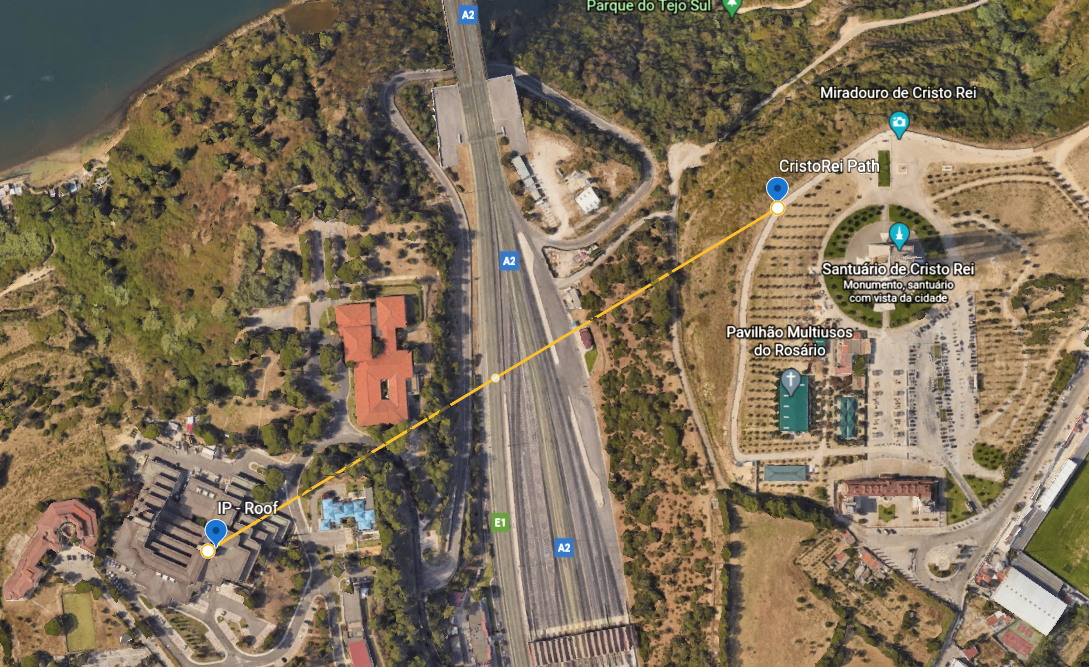
\includegraphics[width=0.8\linewidth]{img/png/experimentMap.png}
    \caption{Location of observer points for the physical experiment.}
    \label{fig:experiment_map}
\end{figure}

The goal of the experiment was to compare passive and active \gls{DOAS}
measurements performed with a very short time difference between them.
The passive measurement would employ the same acquisition strategy as
the drone is expected to use. This comparison will be used to test our
second hypothesis.

Finding two appropriate experiment sites proved to be the first
difficulty: both telescopes should see sky on the back of the other
telescope. Otherwise, the contribution from the terrain's reflection
would have to be taken into account and the experiment conditions would
be very different from the ones the drone will have. There are not many
site pairs that provide this, and most of the ones that exist are
private and authorisations are not easy to obtain. In the end, we
managed to run the experiment in the facilities of \emph{Infraestruturas
de Portugal} and the \emph{Cristo-Rei} sanctuary, near our own base. 

The experiment involved two different optical assemblies, which are
summarised in Table~\ref{tab:assemblies}. Both assemblies play two
roles, which reflect the comparison between active and passive that is
the entire aim of the test. As material in Table~\ref{tab:assemblies}
might imply, the West bank assembly acts as the emitter for the active
mode experiment, while the East bank only plays the part of receiver.

\begin{figure}[htpb]
    \centering
    \caption{Summary table for the two experiment assemblies. Note the
    difference in terms of material, due to the two different roles both
    assemblies play during the experiment.}
    \label{tab:assemblies}
    \missingfigure{}
\end{figure}


The idea of the experiment is as follows. On the night before the
experiment, all equipment is transported onto both sites, and all
alignments are verified and corrected. The experiment starts in the
early morning. Spectral measurements are conducted on both modes,
periodically and with the least amount of time between them. On the
active mode, the light source is collimated by the emitting telescope
and pointed at the receiver. The spectrometer on the East side
continuously takes spectra for 1 minute every 15. When this is over, the
East telescope is pointed towards the opposite direction (which is the
same direction as the emitter telescope) and both the West and East
bank assemblies perform the passive experiment. These are also performed
during 1 minute every 15. We do this 4 times per hour, from half an hour
before sunrise until 11:00 am. Since there is a busy road in between
(arguably the busiest highway section in the country in this period of
the day), we expect to be able to compare pollutant concentrations taken
with both methods, and we expect them to be similar. A schematic
representation of the experiment stages can be found in
Figure~\ref{fig:experiment_schematic}.
\begin{figure}[htpb]
    \centering
    \missingfigure{}
    \caption{Schematic representation of the two types of measurement
    intended for the experiment. On the left the active mode; on the
    right the passive mode.}
    \label{fig:experiment_schematic}
\end{figure}
